\begin{align}
    \because \vec{P} = r\myvec{\cos Q\\ \sin Q}, \vec{Q} = \myvec{0\\0}, \vec{R} = \myvec{p\\0}
    \end{align}
    from the given information, 
    \begin{align}
    \vec{P} = 3\myvec{\cos60\\ \sin60} = \frac{3}{2}\myvec{1\\\sqrt3},  \vec{Q} = \myvec{0\\0},  \vec{R} = \myvec{5.5\\0}
    \end{align}
and plotted in Fig.              \ref{constr/july/1Figure}.
    
    
\begin{figure}[!ht]
\centering
         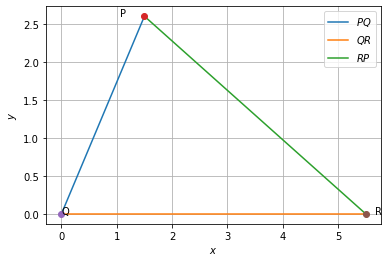
\includegraphics[width= \columnwidth]{solutions/july/2/1/figure1.png}
         \caption{The Constructed triangle}
         \label{constr/july/1Figure}
\end{figure}





